%%
%% Author: maximelovino
%% 2019-06-24
%%

% Preamble
\documentclass[11pt]{article}
\setlength{\parindent}{0pt}
\addtolength{\hoffset}{-3cm}
\addtolength{\textwidth}{6cm}

\addtolength{\voffset}{-2cm}
\addtolength{\textheight}{4cm}

% Packages
\usepackage{amsmath}
\usepackage{url}
\usepackage{graphicx}
\usepackage{float}
\title{Wikipedia Web Traffic Forecasting\\Machine Learning on Big Data - HES-SO Master}
\author{Maxime Alexandre Lovino \and Marco Rodrigues Lopes}

% Document
\begin{document}
    \maketitle
    \section{Introduction and project description}
    This project is inspired by a competition posted by Google on Kaggle\footnote{\url{https://www.kaggle.com/c/web-traffic-time-series-forecasting/}} and is based around the idea of forecasting time series values. For this project, we drew inspirations by submissions from other competitors on Kaggle as well as the work of \emph{JEddy92} on GitHub\footnote{\url{https://github.com/JEddy92/TimeSeries_Seq2Seq}} which inspired our use of the WaveNet model for this project.\\

    Time series are used in multiple domains, the most well known being the stock market values, so we could apply the same type of models to predict stock market changes and become rich....But in practice it would actually be more efficient to use external factors such as trending topics or news articles to find correlations with the changes in the time series.\\

    In this project, we didn't have only one time series to predict but actually a lot of them. 145000 different time series were provided spanning 2.5 years with a granularity of 1 day. The goal of the project is to predict the values for each of them for 60 days in the future. For this project, we didn't use external data to help us with the predictions and relied solely on the time series themselves to predict future values.
    \newpage
    \section{Data description}
    The dataset that can be downloaded on Kaggle consists of two training files in the CSV format and other files which are not relevant to our problem as they're only used for actually submitting an answer for the competition. The two training files consists of the same set of 145000 pages and the same starting date but the second one:\verb+train_2.csv+ is longer, spanning almost 803 days. We decided to use the longer for our experiment has it contains at least two complete years of data. The CSV file weighs 400 MB uncompressed.\\

    The structure of the file consists of a first column containing the page information concatenated in a string, with the title of the page, the lang, the access type and the agent and then a column for each day with the number of views that the specific page got on that day. Some page have \verb+NaN+ values for view on certain dates and this corresponds to the page not having been created yet on that date or just missing values.

    \begin{figure}[H]
        \centering
        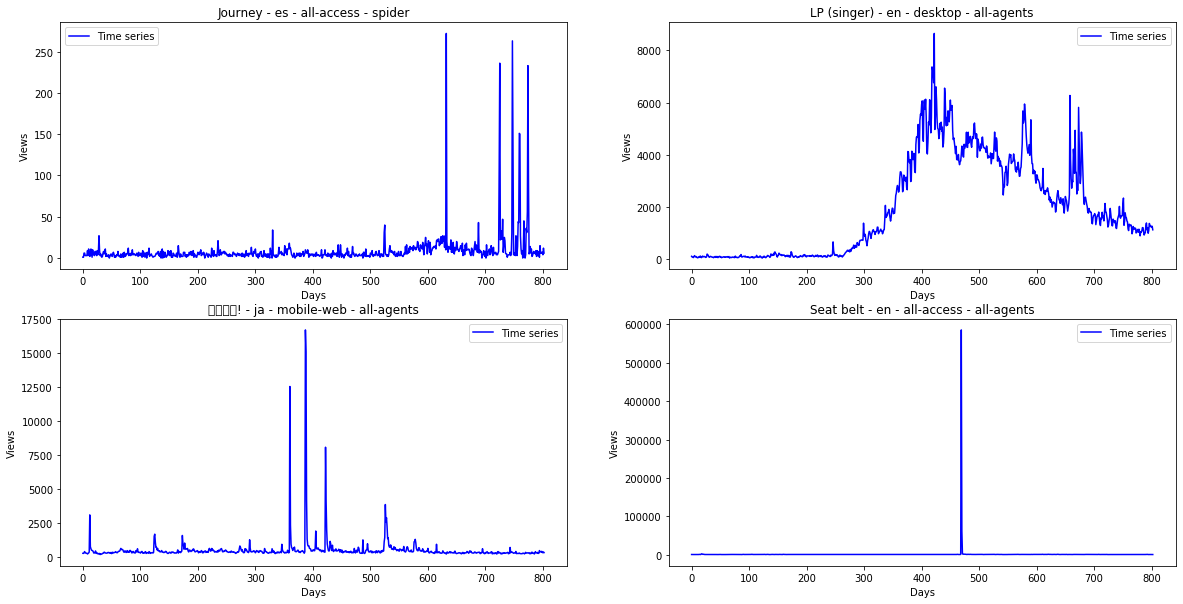
\includegraphics[width=\textwidth]{pages.png}
        \caption{Some of the pages present in the dataset}
    \end{figure}
    \section{Data cleaning and pre-processing}
    The preprocessing and cleaning of the CSV file is handled in the \verb+preprocess_csv_to_pickle+ static method of the \verb+WikiSeries+ classes we have created. This will take a CSV file as an input, extract the information contained in the first column to split in 4 columns (title, lang, access, agent) and remove any page which doesn't belong to a specific country Wikipedia subdomain\footnote{Wikimedia for example}. We will also remove all pages containing \verb+NaN+ values in their series as we can't really replace them with 0 because they didn't actually get 0 views as they didn't exist so we removed them to only work with clean data. After all these steps, we save the resulting Dataframe as a Pickle which will then be used by our other programs. With this cleaning, we reduced our number of pages from 145’063 pages down to 106'328 pages.
    \newpage
    \section{Machine Learning techniques used}
    \subsection{Clustering time series}
    Even with around 100'000 pages down from 145'000 pages, we were still looking for ways to reduce the complexity of the models needed for the datasets so we decided to explore the idea of clustering time series together according to their normalised shapes. In order to do this, we first normalised all time series using min-max scaling for each of them so they had values between 0 and 1. Then we wanted to use Dynamic Time Warping in order to compute a distance between series with small shifts and deformation. The problem is that Dynamic Time Warping computation is complex and it wasn't possible to do it with all pairs from our 100'000 pages.\\

    We selected 1\% of the pages by using stratification from buckets of standard deviation we computed in order to have different types of pages represented in our sampling. We computed DTW distances between pairs of those pages and ran agglomaterive clustering on them. Then we matched all remaining patches to the closest page from the sampling according to the default KNN distance metric.\\

    The resulting clusters were not good enough and not balanced at all, so we abandoned the idea of clustering our series.
    %%\subsection{Light Gradient Boosted Regressor and feature extraction}
    %%TODO if we have space
    \subsection{Deep Learning}
    \subsubsection{Walk forward validation}
    Before training our models, we had to decide how we wanted to split our data. Splitting by pages doesn't make a lot of sense for time series so instead we decided to use Walk Forward validation so that we evaluate the same pages but for a different 60-days windows when evaluating our models. When specifically fitting the model though, we took 40'000 pages and dedicated 20\% for Keras validation so we used a side by side split to fit the model.
    \begin{figure}[H]
        \centering
        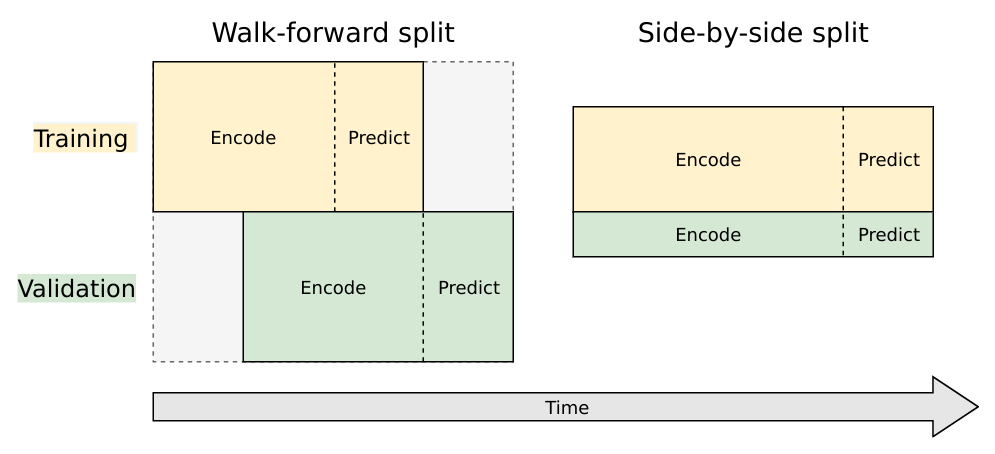
\includegraphics[width=\textwidth]{walkforward.png}
        \caption{Walk forward validation}
    \end{figure}

    \subsubsection{Seq2Seq models}
    \subsubsection{WaveNet}
    \newpage
    \section{Experiments and results}
    \subsection{Training in the cloud}
    \subsection{Evaluating results with SMAPE}
    \subsection{Results for single day predictions}
    \subsection{Results for 60 days prediction}
    \newpage
    \section{Analysis and conclusions}


\end{document}